% Template for ICASSP-2016 paper; to be used with:
%          spconf.sty  - ICASSP/ICIP LaTeX style file, and
%          IEEEbib.bst - IEEE bibliography style file.
% --------------------------------------------------------------------------
\documentclass[12pt]{article}
\usepackage{spconf,amsmath,graphicx,float}
\usepackage{scrlayer-scrpage}
\clearpairofpagestyles
\cfoot*{\pagemark}
% Example definitions.
% --------------------
\def\x{{\mathbf x}}
\def\L{{\cal L}}

% Title.
% ------
\title{Predict the Housing Prices in Ames Report}
%
% Single address.
% ---------------
\name{Atom Group: Jifu Zhao (jzhao59), Jinsheng Wang (jwang278)}
\address{Nuclear, Plasma, and Radiological Engineering \\
              University of Illinois at Urbana-Champaign\\
		       Urbana, Illinois 61801, USA}

\begin{document}
%\ninept
%
\maketitle

\section{Introduction}
\quad\ In this project, our goal is to predict the final price of houses in Ames, Iowa. The data provided by Kaggle were collected in Ames between 2006 and 2010, which contains 79 explanatory variables about the local houses. The given training dataset has 1460 records in total, in which there are 43 categorical variables and 36 numerical variables. 

In this project, we first explore the given training data set. Through some pre-processing methods such as one-hot-encoding and log-transformation, we finally get 287 features with some dummy vairables. Finally, we applied several different models such as Simple Linear regression, Lasso regression and Random Forest on the new feature space and predict those house prices. More details will be described in the following sections.

\section{Pre-processing}
\quad\ After exploring the training dataset, the first thing we noticed is that, there are a lot of missing values for some features, and a summary of those missing values is shown in Table \ref{table}.

\begin{table}[htb]
 \caption{Summary of Missing Values} \label{table}
\begin{center}
  \begin{tabular}{  c  c  c }
    \hline
    Feature Name & Data Type & \# of Missing\\ \hline
    LotFrontage    & integer     & 259 \\
    Alley                & factor    & 1369 \\
    MasVnrType    & factor        & 8 \\
    MasVnrArea    & integer        & 8 \\
    BsmtQual        & factor        & 37 \\
    BsmtCond        & factor        & 37 \\
    BsmtExposure    & factor       & 38 \\
    BsmtFinType1    & factor        & 37 \\
    BsmtFinType2    & factor        & 38 \\
    Electrical            & factor        & 1 \\
    FireplaceQu        & factor        & 690 \\
    GarageType        & factor       & 81  \\
    GarageYrBlt        & integer        & 81 \\
    GarageFinish        & factor        & 81 \\
    GarageQual        & factor        & 81 \\
    GarageCond        & factor        & 81 \\
    PoolQC                & factor        & 1453 \\
    Fence                & factor        & 1179 \\
    MiscFeature        & factor        & 1406 \\
    \hline
  \end{tabular}
\end{center}
\end{table}

From Table \ref{table} we can see that, there are 6 features whose missing value counted more than $15\%$ of the total training set. So, our of first step of pre-processing is to drop those 6 features, namely, LotFrontage, Alley, FireplaceQu, PoolQC, Fence and MiscFeature. 

After dropping those 6 features, for other features that still have missing values, we do the following processing: for numerical values, we replace the missing values with the median of that feature in total training set, and the same procedure was applied to test set. For those categorical data which has missing values, we add a new level of NA for each categorical feature. Then, for those categorical feature, it is not a good idea to directly transform them into numerical variables. A better idea is to transform them into vectors with dummy variables using one-hot-encoding methods. 

After finishing above feature processing, our feature space expands into 287 features in total. With all of these 287 features, we can apply a lot of different models. In this project, we have tried Linear regression, Ridge regression, Lasso regression, xgboost model, random forest model and GBM model. After comparing the performance and running time of each model through cross-validation, we finally choose three models: Simple Linear regression, Lasso regression and Random Forest.

\section{R Library used}
\quad\ In our R code, we loaded five libraries to simplify our task. 'dummy' library was used to generate dummy variables for features with factor values. 'DAGG' was used to help with cross-validation of Linear Regression model. 'randomForest' was introduced to apply random forest technique. 'glmnet' was added to facilitated Lasso regression. Finally, 'moments' had the function that can calculate skewness of features to judge whether long tails exist and apply log transformation if necessary.

\section{Methods}

\subsection{Linear Regression}
\quad\ Within Linear Regression, we fitted a simple linear model that includes all the features generated above. During our experiment, we find that, linear regression model is easy and fast to implement. 3:1 split of training data as train and test only took 1.3 s to run. But the result is not as good as other advanced models shown below.

\subsection{Lasso Regression}
\quad\ In Lasso regression, the best choice of lambda is determined through 10-folder cross-validation and choose the lambda that minimize the cross-validation error. Using all original training and tesing data, the best lambda would be about 0.003 for one run. In fact, we set our Lasso model to automatically generate and use the best lambda according to input training dataset. Lasso model runs very fast with only 1.24 s per trial. Different dataset would end up with different lambda's. This is something similar to online training and prediction. During our experiment, we noticed that Lasso model performed pretty good.

\subsection{Random Forest Model}
\quad\ In random forest model, we used 'randomForest' library and  applied 500 trees to build model. Due to the large amount of trees, this model run very slow, on average each trial would take 25 s. Results showed that in terms of mean square error, random forest model performed better than simple linear model but not as good as Lasso regression.

%\begin{figure}[htb]
%\centering
%\includegraphics[width=8.5cm]{./figures/autoencoder.pdf}
%\caption{Illustration of auto-encoder system.}
%\label{fig:autoencoder}
%\end{figure}

\section{Code Description}
\quad\ All of our code is contained in the file named mymain.R. There are basically three parts in the R file. At the very beginning, the code will automatically check whether or not the required packages/libraries are already installed. In the second part of the code, we do data preprocessing: first read the training and test data sets, then drop the useless variables and process the features to form the new feature space. For the last part, we mainly build our three model: Linear Regression, Lasso Regression and Random Forest model. These built models will make predictions and the results are saved into local file system as required by the project description.

\section{Results}

\quad\ To test our models, we randomly chose 75\% of data in train.csv as the training set, then use the rest 25\% of data as the test set. This process was repeated 5 times to calculate the average running time, mean-square-error and standard deviation of MSE (MSE is calculated based on log scale) for each model. The result of 5 runnings is shown in Figure \ref{fig:autoencoder}.

\begin{figure}[htb]
\centering
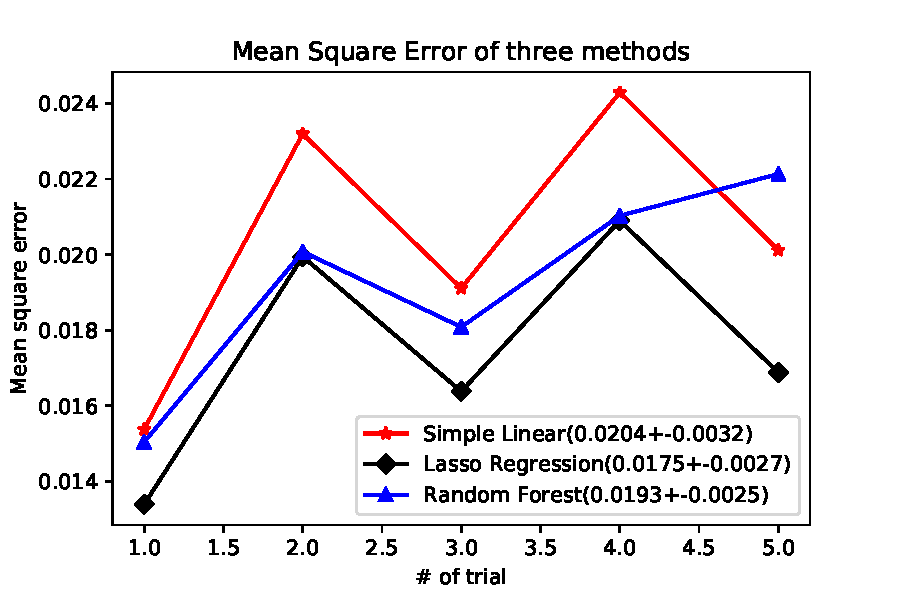
\includegraphics[width=0.45\textwidth]{./figures/MSE_3_methods.pdf}
\caption{Results of different models}
\label{fig:autoencoder}
\end{figure}

The running time mean, MSE mean and standard deviation of MSE are shown in Table \ref{result}.

\begin{table}[htb]
 \caption{Summary of Models} \label{result}
\begin{center}
  \begin{tabular}{  c  c c  c }
    \hline
    Model                             &Time mean(s)              & MSE mean    & MSE std \\ \hline
    Linear Regression           & 1.3126                               & 0.0204      & 0.0032 \\
    Lasso Regression                & 1.2413                          & 0.0175    & 0.0027 \\
    Random Forest                  & 25.6746                          & 0.0193          & 0.0025 \\
    \hline
  \end{tabular}
\end{center}
\end{table}

From Table \ref{result}, one can find that, our Lasso model performed best, while linear regression model performed worst. Lasso and Linear models run very fast while random forest will take much longer time. At the end, we applied our models to kaggle data and uploaded our predictions, Lasso submission ranked highest among the three models, with a 1708/4810 ranking.

\subsection*{Acknowledgement}

\quad\ The authors would like to thank Xichen Huang for his tutorial notebook on Piazza. Our code borrowed some of the data pre-processing methods from his class R code session.

\vfill\pagebreak

% References should be produced using the bibtex program from suitable
% BiBTeX files (here: strings, refs, manuals). The IEEEbib.bst bibliography
% style file from IEEE produces unsorted bibliography list.
% -------------------------------------------------------------------------
%\bibliographystyle{IEEEbib}%\bibliography{strings,refs}
%\bibliography{strings}

\end{document}
